%falar de o termo AM supervisionada
%fazer orcamento
\section{Introdução e Motivação}
Atualmente, o aprendizado de máquina permeia o cotidiano humano
provendo auxílio em tarefas diversas \citep{Bishop2006}.
Seu bom desempenho na tarefa de classificação depende da existência de dados
categorizados de qualidade para treinamento do sistema e de um algoritmo de
aprendizado adequado.
A categorização dos dados é um processo frequentemente custoso,
pois é realizada por um supervisor humano que atribui categorias/classes para cada
objeto/exemplo de interesse contido nos dados ou, dependendo da aplicação,
é realizada por um processo químico ou mecânico \citep{journals/etai/BryantMOKRK01},
por exemplo.

Dados os limites práticos de orçamento, esforço humano disponível, resistência à fadiga
e crescente presença massiva de dados, faz-se necessária a \textit{amostragem} de
apenas um subconjunto de exemplos para a rotulação e subsequente construção do
conjunto de treinamento.
Quando se deseja eficiência no uso de recursos, essa amostragem de exemplos não é trivial,
pois resultados teóricos e empíricos apontam para a existência de uma diferença de
desempenho entre os métodos desenvolvidos na área de \textit{aprendizado ativo}
\citep{series/synthesis/2012Settles} frente à amostragem aleatória.
Apesar de ser uma área promissora, a diversidade de métodos de amostragem
ativa aliada às diferentes características de cada base de dados e aos vieses dos algoritmos
de aprendizado dificulta a fase de projeto de um sistema de aprendizado de máquina.
Existem assim, dois problemas de escolha: estratégia de amostragem e algoritmo
de aprendizado.

Tradicionalmente, a escolha do algoritmo de aprendizado é feita com base na experiência
pessoal do especialista responsável pelo sistema ou em restrições próprias da aplicação.
Outra possibilidade é o uso de um método automático de recomendação como o
\textit{meta-aprendizado} \citep{books/daglib/0022052}.
Apesar dessas abordagens serem indicadas para o caso do aprendizado supervisionado
convencional, em que todos os exemplos de treinamento já estão rotulados,
elas não foram propostas para a situação de escassez ou ausência de rótulos, que é o caso
de aplicações com orçamento limitado e ainda na fase de escolha da melhor forma
de amostragem para rotulação.

Idealmente, a escolha do algoritmo de aprendizado é baseada em métodos de validação
cruzada. Logo, a escolha se dá com o conjunto de treinamento completo, ou seja,
amostrado e rotulado.
Consequentemente, a escolha do estratégia de amostragem ativa,
precede a determinação do algoritmo de aprendizado.
Outra particularidade na escolha da estratégia é
sua criticidade, tendo-se em vista que o sucesso da estratégia escolhida só pode ser
determinado após ter-se incorrido em custos financeiros com a atividade de supervisão.
Dessa forma, é preciso adotar uma estratégia com base em expectativas de desempenho
ou de acordo com características da base de dados.
Na prática, essa escolha tem sido arbitrária, tendendo a se concentrar
no uso da estratégia mais simples, chamada \textit{amostragem por incerteza}.
Essa preferência foi reportada numa competição de aprendizado ativo,
onde também prevaleceu a ausência de estratégias possivelmente mais efetivas
como as baseadas em densidade conforme
Figura \ref{compet}.
\begin{figure}
\caption{Frequência de uso de estratégias na competição de aprendizado ativo
(alguns participantes adotaram mais de uma estratégia).
\textit{Adaptado de \citep{journals/jmlr/GuyonCDL11}.}}
\label{compet}
\begin{center}
    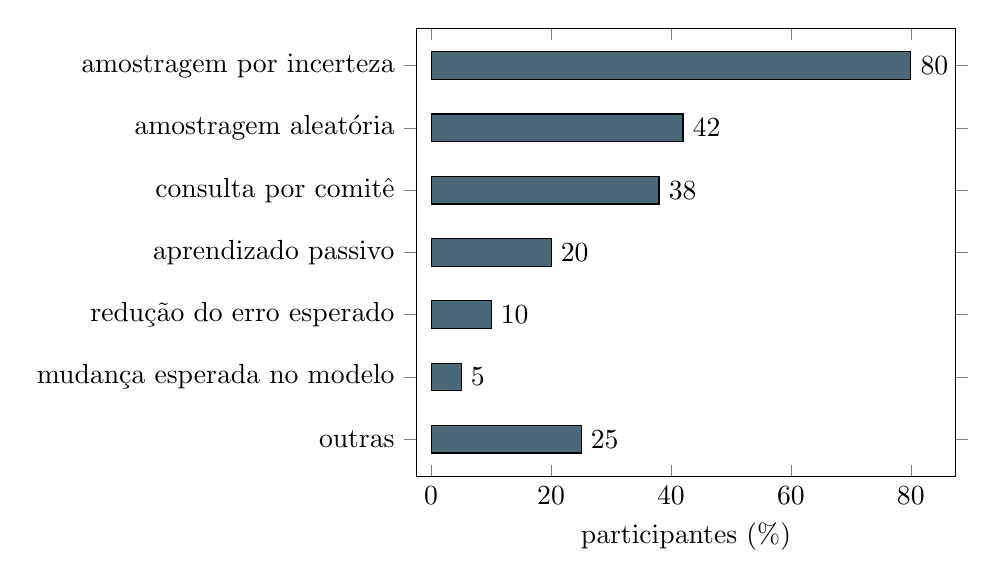
\begin{tikzpicture}
\begin{axis}[
    xbar,
%     xmin=0.0,
%     width=12cm,
%     height=40cm,
%     enlarge x limits={rel=0.13,upper},
    ytick={1,2,3,4,5,6,7},
    yticklabels={
    {amostragem por incerteza},
    {amostragem aleatória},
    {consulta por comitê},
    {aprendizado passivo},
    {redução do erro esperado},
    {mudança esperada no modelo},
    {outras}
    },
%         enlarge y limits=0.4,
    xlabel={participantes (\%)},
    ytick=data,
    nodes near coords,
    nodes near coords align=horizontal
]
\addplot [draw=black, fill=cyan!40!black] coordinates {
    (80,7)
    (42,6)
    (38,5)
    (20,4)
    (10,3)
    (5,2)
    (25,1)
};
\end{axis}
\end{tikzpicture}
\end{center}
\end{figure}
% challenge:
% global_score = (ALC-Arand)/(Amax-Arand)       Amax = 1
% semi-supervised learning is needed to achieve good performance in the first part of the learning curve
% (usar ou não semisupervised é um problema à parte, que faz parter do learner, não da estratégia; classificadores semisupervisionados são melhores, mas não é isso que se está avaliando quando se comparam estratégias; ensembles, feature selection e SMOTE também ajudam e nem por isso precisam ser empregados na comparação de estratégias)
Em consonância com esse panorama, está a ausência de estudos comparativos
abrangentes que possam guiar o especialista na fase de amostragem.
% - até onde o conhecimento do autor permite dizer -

Adicionalmente, diversas estratégias fazem uso interno de algoritmos de aprendizado para
embasar a amostragem.
Esse uso interno fecha um círculo impossível de dependências:
a estratégia depende do algoritmo; o algoritmo depende da existência do conjunto
de treinamento que requer rotulação; e,
a rotulação é feita pela estratégia de aprendizado ativo.
A forma trivial de se evitar o círculo de dependências, para além da amostragem aleatória,
é a adoção de estratégias agnósticas.
Essas estratégias não fazem suposições a respeito dos dados no que diz respeito ao viés de
aprendizado, pois não requerem um algoritmo interno.
Elas se baseiam, por exemplo, em medidas de densidade ou estatísticas de agrupamento
\citep{journals/tcs/Dasgupta11}.
A dispensa do algoritmo, entretanto, leva a amostragens que não consideram a fronteira
de decisão que seria traçada durante o aprendizado.
Ela contém informações que permitem consultas mais prospectivas que exploratórias,
potencialmente acelerando a descoberta dos exemplos mais relevantes.

Assim, existem pelo menos dois problemas e respectivos subproblemas em aberto na área
de aprendizado ativo:
\begin{itemize}
 \item Que situações dispensam o uso de aprendiz (algoritmo interno)?
 Dentre as estratégias agnósticas, qual a mais indicada para um dado problema?
 \item Como quebrar o círculo de dependências?
 Dentre as estratégias gnósticas, qual a mais indicada para um dado problema?
\end{itemize}

Neste projeto, propõe-se investigar os desdobramentos da aplicação de meta-aprendizado como apoio 
na definição do melhor par estratégia-algoritmo.
Essa forma de recomendação automática quebra o círculo de dependências, pois o aprendiz é recomendado em
conjunto com a estratégia, isentando o usuário de definir um algoritmo compatível com
ambas, base de dados e estratégia.
Está implícito nessa abordagem que o algoritmo de aprendizado do aprendiz é desvinculado
do algoritmo de aprendizado do classificador definitivo da aplicação.
O algoritmo do classificador definitivo é escolhido apenas após a rotulação.

O meta-aprendizado tem sido investigado e demonstrado efetivo no grupo de pesquisa
do candidato na melhoria da classificação de dados de expressão gênica
\cite{souza2010c,souza2010b,souza2009,1442541}.
O presente enfoque é verificar sua aplicabilidade na recomendação de estratégias e algoritmos
bisando uma rotulação eficiente.

 Este plano de pós-doutorado é organizado como segue.
 Na Seção \ref{aa}, os principais paradigmas de aprendizado ativo são expostos.
Uma introdução ao meta-aprendizado é apresentada na Seção \ref{ma}.
Finalmente, na Seção \ref{pr}, a proposta é detalhada juntamente com o plano de atividades e recursos necessários.
